\chapter{Pinbelegung}
\label{ch:Pinbelegun}
%% ==============================
Anhang A\ldots

\section{Tex Beispiele}
\subsection{Zitieren}
Quellen\cite{li00,jackson91,lakhina04a,netflow,rfc2386} 
nicht vergessen. Dazu verwendet ihr bibtex.


\subsection{Ein Bild skaliert}

\begin{figure}[htbp]%Positionierung vorzugsweise an dieser Stelle. Falls nicht möglich oben positionieren. Falls das auch nicht geht unten.
	\centering
		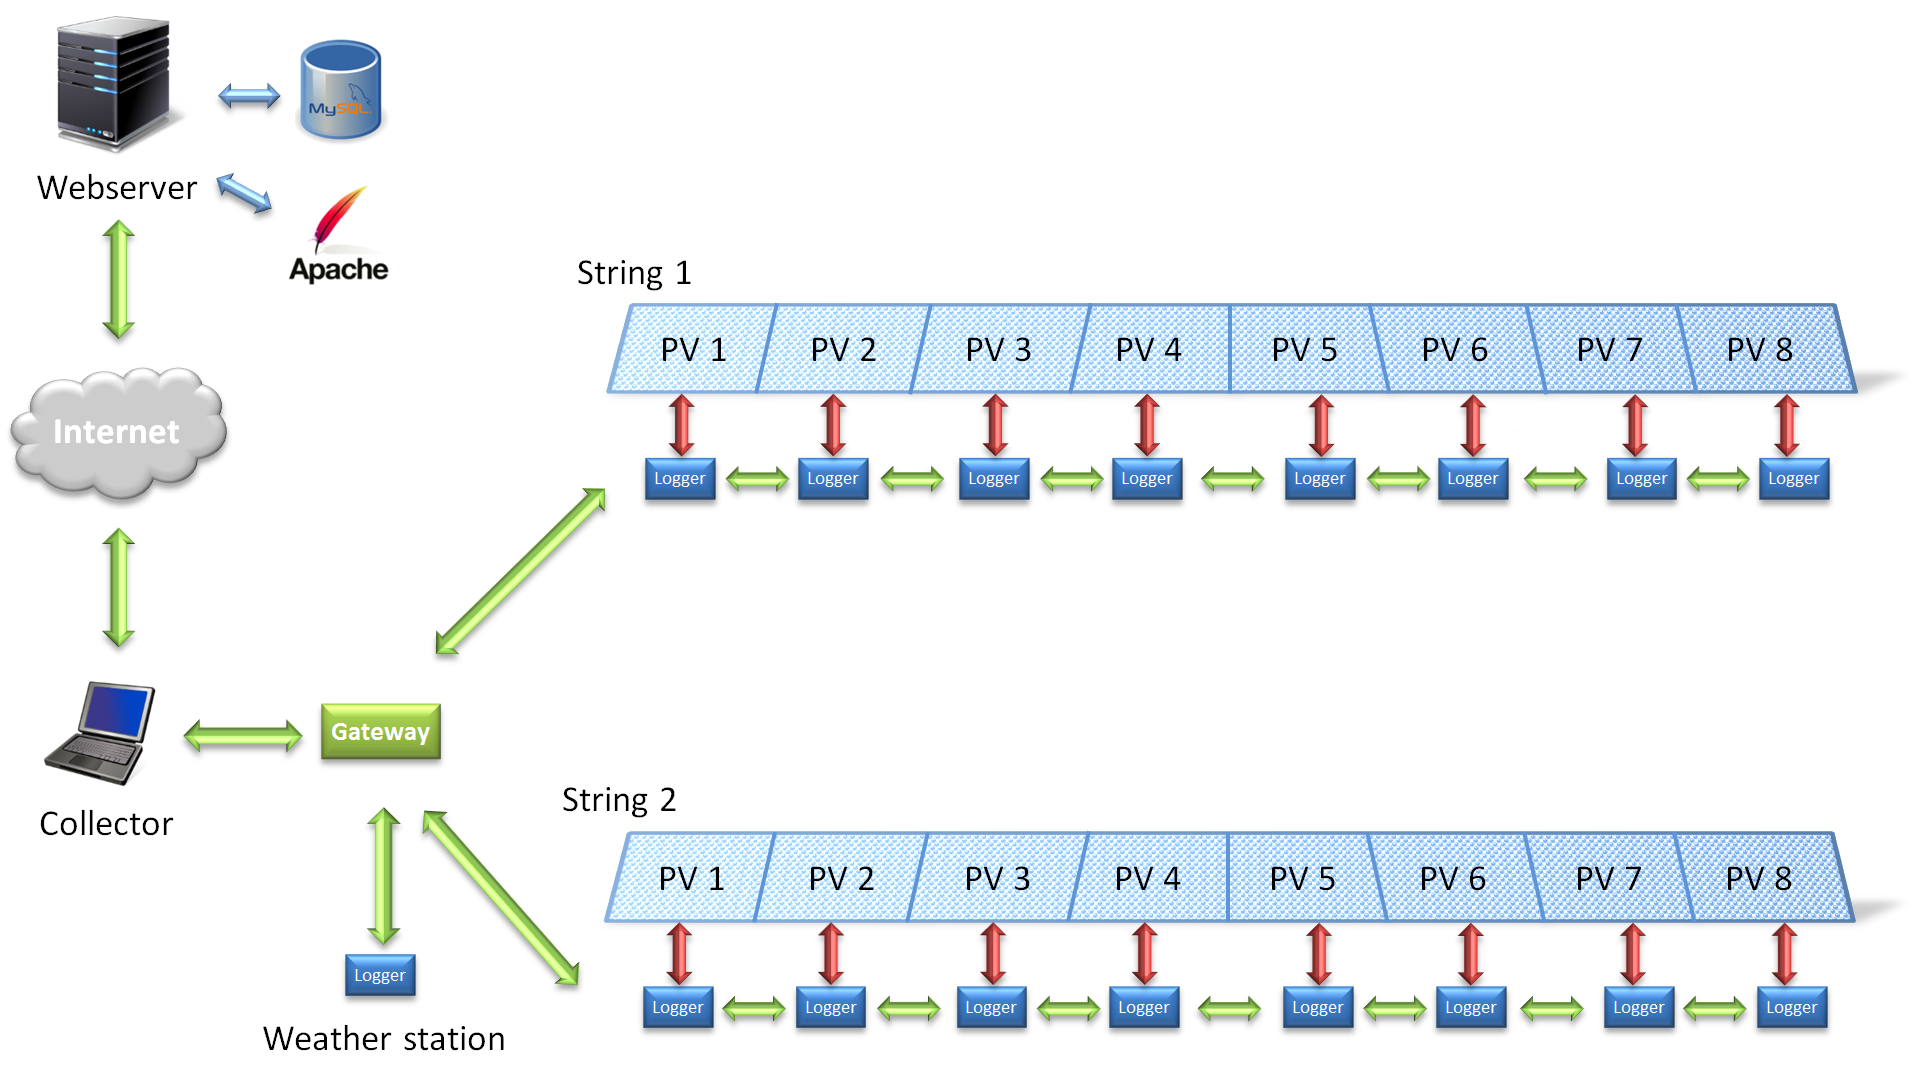
\includegraphics[width=0.80\textwidth]{../figures/large1.png}
	\caption{Beschriftungstext}
	\label{fig:large1}
\end{figure}

\subsection{Zwei Bilder nebeneinander oder untereinander}
\begin{figure*}[!htb]
	\centering
	\subfigure[Beschriftung Bild links]{
	  \label{fig:small1}
		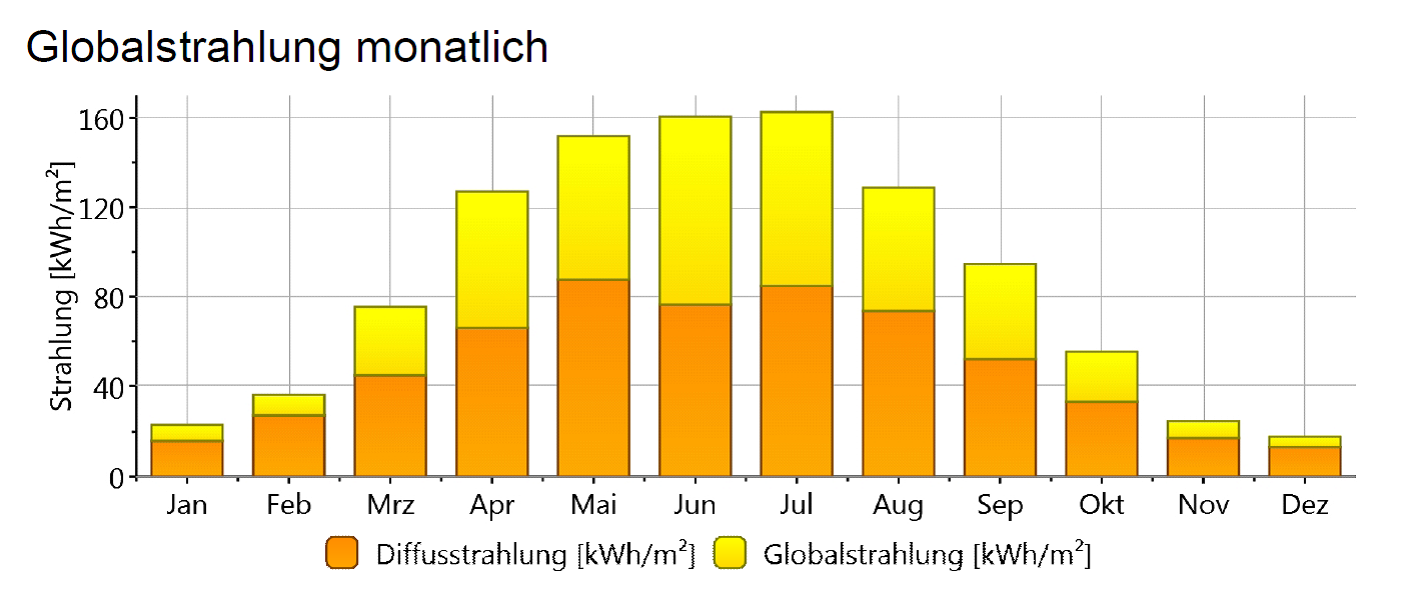
\includegraphics[angle=0,width=0.68\textwidth]{../figures/small1.png}}
	\subfigure[Beschriftung Bild rechts]{
	  \label{fig:small2}
		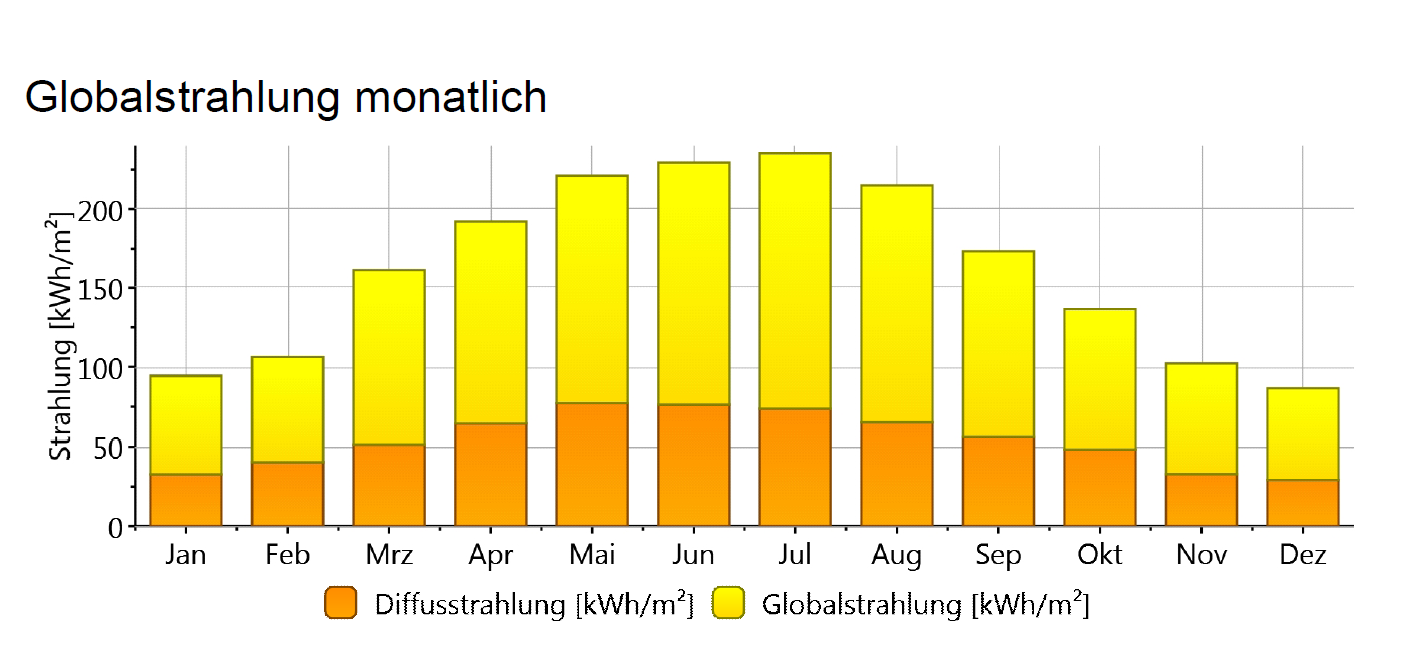
\includegraphics[angle=0,width=0.68\textwidth]{../figures/small2.png}}
 	\caption{Beschriftung beide Bilder} 
	\label{fig:beidebilder}
\end{figure*}


\section{Tabellen}


\begin{table}[htb]
		\centering
		%\renewcommand{\arraystretch}{1.03}
		\caption{Single-hop Scenario - Traffic Pattern \label{t:traffic}}
			
		\begin{tabular}{l@{~}l@{\,\,}l@{\,\,}l} \hline \rule{-2pt}{12pt}
			Pattern& Parameter & Distribution & Range/Values  \rule{0pt}{12pt} \\ \hline \rule{-2pt}{12pt}  
      \textbf{Burst}      
      & Burst IAT         & uniform  & [9.9; 10.1] s\\ 
      & Packets per Burst & constant & 100\\
      & Packet IAT        & constant & 0.02 s\\
      & Packet Size       & constant & 1024 bit\\
      & \# Sources & -        & 2\\
			& Offset						& uniform  & [0; 1] s\\ 
      \hline      \hline\rule{-2pt}{12pt} 
      \textbf{Single}     & Packet IAT        & uniform  & [0.9; 1.1] s\\
      & Packet Size       & constant & 1024 bit\\
      & \# Sources & -        & [10;20;30;40;50;\\
      & & & 60;70;80;90;100]\\
			& Offset						& uniform  & [0; 1] s\\ 
      \hline
    \end{tabular}
\end{table}
